\section{Supplementary Figures}
\begin{figure}
    \centering{
        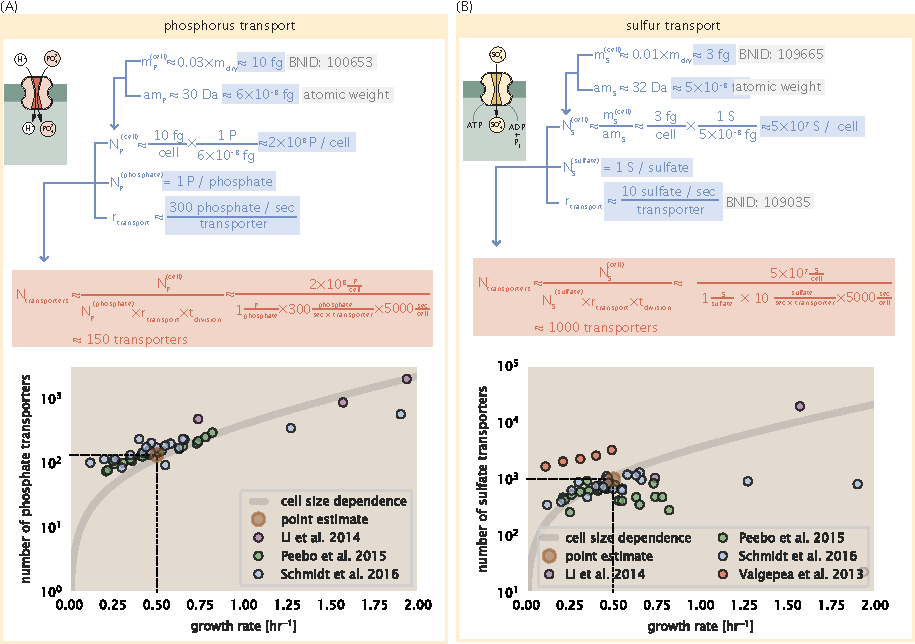
\includegraphics{main_figs/fig2-S1_phospho_sulfo_transport.pdf}
        \caption{\textbf{Estimates and observed abundances of phosphate and sulfate transporters.}(A) Estimate for the number of PitA
    phosphate transport systems needed to maintain a 3\% phosphorus \textit{E.
    coli} dry mass. Points in plot correspond to the total number of PitA
    transporters per cell. (B) Estimate of the number of CysUWA complexes
    necessary to maintain a 1\% sulfur \textit{E. coli} dry mass. Points in plot
    correspond to average number of CysUWA transporter complexes that can be
    formed given the transporter stoichiometry [CysA]$_2$[CysU][CysW][Sbp/CysP].
    Grey line in (A) and (B) represents the estimated number of transporters per
    cell at a continuum of growth
    rates.}\label{fig:phospho_sulfo}
    }
\end{figure}    

\begin{figure}
    \centering{
    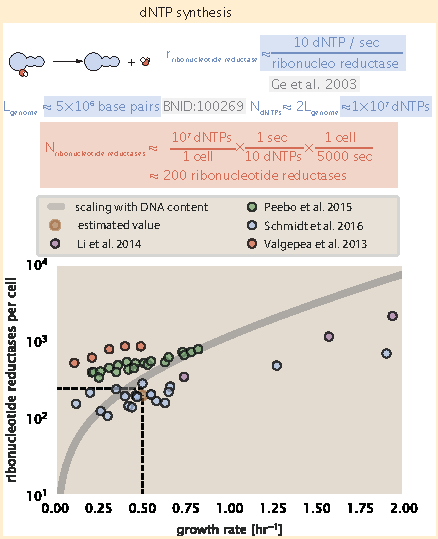
\includegraphics[scale=0.9]{main_figs/fig7-S1_dNTP_synthesis.pdf}
    \caption{\textbf{Estimate and observations of the abundance of ribonucleotide
    reductase, a key component in dNTP synthesis.}Estimate of the number of
    ribonucleotide reductase enzymes needed to facilitate the synthesis of
    $\approx 10^7$ dNTPs over the course of a 5000 second generation time. Points
    in the plot correspond to the total number of ribonucleotide reductase I
    ([NrdA]$_2$[NrdB]$_2$) and ribonucleotide reductase II ([NrdE]$_2$[NrdF]$_2$)
    complexes. Grey lines in top panel show the estimated number of complexes
    needed as a function of growth, the details of which are described in the
    Appendix.}\label{fig:dntp}
    }
\end{figure}

\begin{figure}
    \centering{
    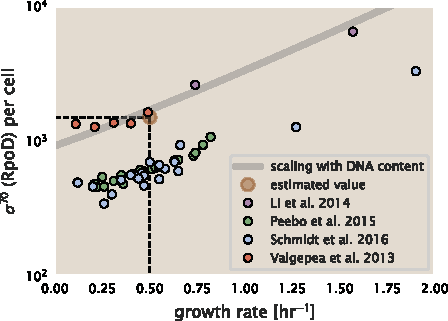
\includegraphics[scale=0.9]{main_figs/fig8-S1_sigma_factor.pdf}
        \caption{\textbf{Abundance and growth rate dependence of
        $\sigma$-70.} The abundance of $\sigma^{70}$ as a function of growth
        rate. Estimated value for the number of RNAP is shown as a
        translucent brown point and grey line.} \label{fig:sigma_70}
   }
\end{figure}


\begin{figure}
    \centering{
    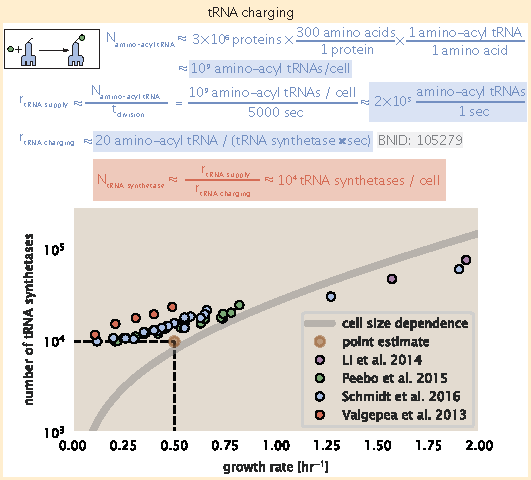
\includegraphics{main_figs/fig9-S1_tRNA.pdf}
    \caption{\textbf{Estimate and observed abundance and growth rate dependence
        of tRNA ligases.}Estimation for the number of tRNA synthetases that
        will supply the required amino acid demand. The sum of all tRNA
        synthetases copy numbers are plotted as a function of growth rate
        ([ArgS], [CysS], [GlnS], [GltX], [IleS], [LeuS], [ValS], [AlaS]$_2$,
        [AsnS]$_2$, [AspS]$_2$, [TyrS]$_2$, [TrpS]$_2$, [ThrS]$_2$,
        [SerS]$_2$, [ProS]$_2$, [PheS]$_2$[PheT]$_2$, [MetG]$_2$,
        [lysS]$_2$, [HisS]$_2$, [GlyS]$_2$[GlyQ]$_2$).}
        \label{fig:tRNA}
        }
    
\end{figure}

\begin{figure}
    \centering{
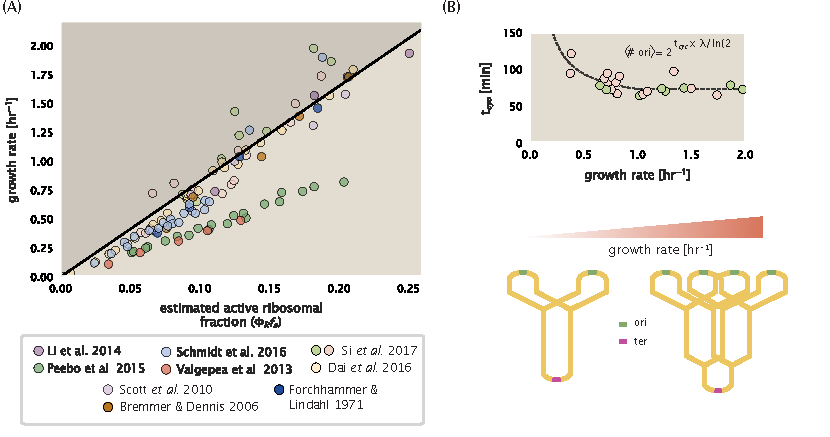
\includegraphics[scale=0.9]{main_figs/fig10-S1_ribosome_as_limit.pdf}

\caption{\textbf{Comparison of $\Phi_R f_a$ with literature and estimation of
        $\langle$\# ori$\rangle$.}(A) Actively translating ribosomal
        fraction versus growth rate. The actively translating ribosomal
        fraction is calculated using the estimated values of $f_a$ from
        \cite{dai2016} (shown in inset; see the Appendix Section
        "Calculation of active ribosomal fraction for
        additional detail). Additional measurements in addition to the
        proteomic measurements are based on measurements of cellular RNA to
        protein ratio, with $\Phi_R \approx$ the cellular RNA to protein
        ratio divided by 2.1 \citep{dai2016}. (B) Experimental measurements
        of the cell doubling time $\tau$ and cell cycle time $t_{cyc}$ from
        Si \textit{et al.} (2017). Dashed line shows fit to the data, which
        were used to estimate $\langle$\# ori$\rangle$. $t_{cyc}$ was assumed
        to vary in proportion to $\tau$ for doubling times greater than 40
        minutes, and reach a minimum value of 73 minutes. See Appendix
        Section "Estimation of $\langle$\# ori$\rangle$ / $\langle$\# ter$\rangle$ and $\langle$\# ori$\rangle$" for additional details exact estimation of rRNA
        copy number. Red data points correspond to measurements in strain
        MG1655, while light green points are for strain NCM3722. Schematic
        shows the expected increase in replication forks (or number of ori
        regions) as \textit{E. coli} cells grow faster.} \label{fig:ribosome_limit_supp}
   }
\end{figure}


\begin{figure}    
    \centering{
   \includegraphics[scale=0.4]{main_figs/fig12-S1_model_explorer_screenshot.png}
   \caption{\textbf{An interactive figure for exploration of the model parameter
    space.} An interactive version of parts (B) and (C) of
    Figure \ref{fig:elongation_rate_model} which permit the user to modulate the rate
    of amino acid supply, the dissociation constant of amino acids to the
    ribosome, and the fraction of the ribosome pool that is actively
    translating. This interactive figure, and the code used to generate it,
    is available on the \href{https://rpgroup.caltech.edu/growth_limit}{paper website.}}
    \label{fig:model_explorer}
    }
\end{figure}